\documentclass[a4paper,11pt]{article}
\usepackage{amsmath,amsthm,amsfonts,amssymb,amscd,amstext,vmargin,graphics,graphicx,tabularx,multicol} 
\usepackage[francais]{babel}
\usepackage[utf8]{inputenc}  
\usepackage[T1]{fontenc} 
\usepackage{pstricks-add,tikz,tkz-tab,variations}
\usepackage[autolanguage,np]{numprint} 

\setmarginsrb{1.5cm}{0.5cm}{1cm}{0.5cm}{0cm}{0cm}{0cm}{0cm} %Gauche, haut, droite, haut
\newcounter{numexo}
\newcommand{\exo}[1]{\stepcounter{numexo}\noindent{\bf Exercice~\thenumexo} : \marginpar{\hfill /#1}}
\reversemarginpar


\newcounter{enumtabi}
\newcounter{enumtaba}
\newcommand{\q}{\stepcounter{enumtabi} \theenumtabi.  }
\newcommand{\qa}{\stepcounter{enumtaba} (\alph{enumtaba}) }
\newcommand{\initq}{\setcounter{enumtabi}{0}}
\newcommand{\initqa}{\setcounter{enumtaba}{0}}

\newcommand{\be}{\begin{enumerate}}
\newcommand{\ee}{\end{enumerate}}
\newcommand{\bi}{\begin{itemize}}
\newcommand{\ei}{\end{itemize}}
\newcommand{\bp}{\begin{pspicture*}}
\newcommand{\ep}{\end{pspicture*}}
\newcommand{\bt}{\begin{tabular}}
\newcommand{\et}{\end{tabular}}
\renewcommand{\tabularxcolumn}[1]{>{\centering}m{#1}} %(colonne m{} centrée, au lieu de p par défault) 
\newcommand{\tnl}{\tabularnewline}

\newcommand{\trait}{\noindent \rule{\linewidth}{0.2mm}}
\newcommand{\hs}[1]{\hspace{#1}}
\newcommand{\vs}[1]{\vspace{#1}}

\newcommand{\N}{\mathbb{N}}
\newcommand{\Z}{\mathbb{Z}}
\newcommand{\R}{\mathbb{R}}
\newcommand{\C}{\mathbb{C}}
\newcommand{\Dcal}{\mathcal{D}}
\newcommand{\Ccal}{\mathcal{C}}
\newcommand{\mc}{\mathcal}

\newcommand{\vect}[1]{\overrightarrow{#1}}
\newcommand{\ds}{\displaystyle}
\newcommand{\eq}{\quad \Leftrightarrow \quad}
\newcommand{\vecti}{\vec{\imath}}
\newcommand{\vectj}{\vec{\jmath}}
\newcommand{\Oij}{(O;\vec{\imath}, \vec{\jmath})}
\newcommand{\OIJ}{(O;I,J)}


\newcommand{\bmul}[1]{\begin{multicols}{#1}}
\newcommand{\emul}{\end{multicols}}

\newcommand{\reponse}[1][1]{%
\multido{}{#1}{\makebox[\linewidth]{\rule[0pt]{0pt}{20pt}\dotfill}
}}

\newcommand{\titre}[5] 
% #1: titre #2: haut gauche #3: bas gauche #4: haut droite #5: bas droite
{
\noindent #2 \hfill #4 \\
#3 \hfill #5

\vspace{-1.6cm}

\begin{center}\rule{6cm}{0.5mm}\end{center}
\vspace{0.2cm}
\begin{center}{\large{\textbf{#1}}}\end{center}
\begin{center}\rule{6cm}{0.5mm}\end{center}
}



\begin{document}
\pagestyle{empty}
\titre{Contrôle 3}{Nom :}{Prénom :}{Classe}{Date}

\emph{Dans tout le contrôle, une attention particulière sera portée pour faire apparaître un minimum d'étapes correspondants à des règles du cours, ainsi qu'à la propreté et à la rédaction.}\\


\exo{3} Calculer et donner le résultat sous forme de fraction irréductible :\\

\begin{center}
	$A=\displaystyle{\frac{-17}{3}}+\displaystyle{\frac{5}{15}}$ \hspace{20 mm} $B=4+\displaystyle{\frac{-6}{7}}$ \hspace{20 mm}  $F=\displaystyle{\frac{18}{11}}-\displaystyle{\frac{-1}{11}}$ 
\end{center}


\exo{5,5} Calculer et donner le résultat sous forme de fraction irréductible :\\


\begin{center}
	$E=\displaystyle{\frac{5}{14}}\times7$ \hspace{20 mm} $F=\displaystyle{\frac{-2}{3}}\times\displaystyle{\frac{-9}{4}}\times\displaystyle{\frac{8}{-10}}$ \hspace{20 mm}
	\vspace{5 mm}
	$H=\displaystyle{\frac{5}{4}}\div\displaystyle{\frac{3}{7}}$ \hspace{20 mm} 	

	$K=\displaystyle{\frac{\displaystyle{\frac{8}{21}}}{4}}$ \hspace{20 mm} $L=\displaystyle{\frac{-5}{\displaystyle{\frac{-5}{-5}}}}$
\end{center}

\exo{3} Calculer et donner le résultat sous forme de fraction irréductible :\\

\begin{center}
	$M=\displaystyle{\frac{3}{4}}+\displaystyle{\frac{1}{4}}\times\displaystyle{\frac{3}{5}}$ \hspace{20 mm} $N=\displaystyle{\frac{7}{6}}\div\displaystyle{\frac{2}{3}}-\displaystyle{\frac{1}{3}}$ 
\end{center}


\exo{2}

\bmul{2}
On considère la figure ci-contre sur laquelle :
(C ) est un cercle de centre U et de diamètre [RS].
V est le milieu du segment [RT].\\
\textbf{Démontrer que} : les droites (UV) et (ST ) sont parallèles.

\columnbreak

\begin{center}
\includegraphics[scale=1]{cercle.eps} 
\end{center}

\emul


\exo{3}

\bmul{2}

Dans le triangle ADC : M est le milieu de [DA], N est un point de [DC] et (MN) est parallèle à (AC).
Dans le triangle ABC : $\widehat{ABC}$  est droit, AB = 4, 2 cm ; BC = 5, 6 cm et AC = 7,08 cm.

\noindent \q Que peut-on dire du point N ? (\textbf{Démontrer}-le)\\
\q Calculer la longueur du segment [MN].

\columnbreak

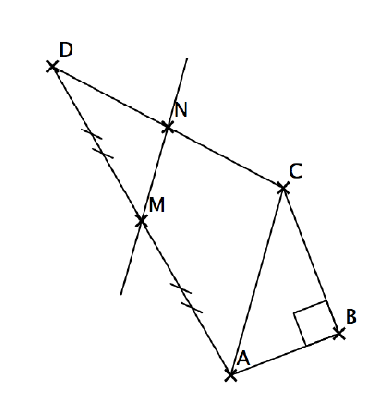
\includegraphics[scale=1]{fig.eps} 

\emul


\exo{3,5}

Dans le triangle EMC, rectangle en C : N est le milieu de [EM] et K est le milieu de [MC].\\

\textbf{Démontrer que} le triangle MKN est rectangle.\\

\begin{center}
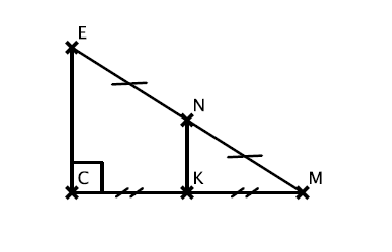
\includegraphics[scale=1]{fig2.eps} 
\end{center}


\exo{1,5} Bonus \\
\initq 

\q Quelle est le résultat de la somme de 1 et de l'inverse de la somme de 1 et de l'inverse de la somme de 1 et 1 ?\\

\q Calculer $O=\displaystyle{\frac{\displaystyle{\frac{1}{2}}+5}{\displaystyle{\frac{1}{5}}-\displaystyle{\frac{1}{10}}}}$










\end{document}
